\documentclass[12pt,letterpaper]{article}\usepackage[]{graphicx}\usepackage[]{color}
%% maxwidth is the original width if it is less than linewidth
%% otherwise use linewidth (to make sure the graphics do not exceed the margin)
\makeatletter
\def\maxwidth{ %
  \ifdim\Gin@nat@width>\linewidth
    \linewidth
  \else
    \Gin@nat@width
  \fi
}
\makeatother

\definecolor{fgcolor}{rgb}{0.345, 0.345, 0.345}
\newcommand{\hlnum}[1]{\textcolor[rgb]{0.686,0.059,0.569}{#1}}%
\newcommand{\hlstr}[1]{\textcolor[rgb]{0.192,0.494,0.8}{#1}}%
\newcommand{\hlcom}[1]{\textcolor[rgb]{0.678,0.584,0.686}{\textit{#1}}}%
\newcommand{\hlopt}[1]{\textcolor[rgb]{0,0,0}{#1}}%
\newcommand{\hlstd}[1]{\textcolor[rgb]{0.345,0.345,0.345}{#1}}%
\newcommand{\hlkwa}[1]{\textcolor[rgb]{0.161,0.373,0.58}{\textbf{#1}}}%
\newcommand{\hlkwb}[1]{\textcolor[rgb]{0.69,0.353,0.396}{#1}}%
\newcommand{\hlkwc}[1]{\textcolor[rgb]{0.333,0.667,0.333}{#1}}%
\newcommand{\hlkwd}[1]{\textcolor[rgb]{0.737,0.353,0.396}{\textbf{#1}}}%

\usepackage{framed}
\makeatletter
\newenvironment{kframe}{%
 \def\at@end@of@kframe{}%
 \ifinner\ifhmode%
  \def\at@end@of@kframe{\end{minipage}}%
  \begin{minipage}{\columnwidth}%
 \fi\fi%
 \def\FrameCommand##1{\hskip\@totalleftmargin \hskip-\fboxsep
 \colorbox{shadecolor}{##1}\hskip-\fboxsep
     % There is no \\@totalrightmargin, so:
     \hskip-\linewidth \hskip-\@totalleftmargin \hskip\columnwidth}%
 \MakeFramed {\advance\hsize-\width
   \@totalleftmargin\z@ \linewidth\hsize
   \@setminipage}}%
 {\par\unskip\endMakeFramed%
 \at@end@of@kframe}
\makeatother

\definecolor{shadecolor}{rgb}{.97, .97, .97}
\definecolor{messagecolor}{rgb}{0, 0, 0}
\definecolor{warningcolor}{rgb}{1, 0, 1}
\definecolor{errorcolor}{rgb}{1, 0, 0}
\newenvironment{knitrout}{}{} % an empty environment to be redefined in TeX

\usepackage{alltt}
\usepackage[utf8]{inputenc}
\usepackage[margin=.7in]{geometry}
\usepackage{graphicx}
\usepackage{titling}
\usepackage{amsmath}
\usepackage{amsfonts}
\usepackage{amssymb}
\renewcommand{\theenumiv}{\arabic{enumiv}}
\setlength{\droptitle}{-5em}
\author{Maurice Diesendruck\vspace{-2ex}}
\title{StatMod2 - Hierarchical Models and Shrinkage - Exercises 4\vspace{-1ex}}
\IfFileExists{upquote.sty}{\usepackage{upquote}}{}
\begin{document}
\maketitle

\section{School Averages and Sample Size}

Larger samples tend to "smooth" out extreme scores, so small samples are more 
likely to be extreme.\\

\begin{knitrout}
\definecolor{shadecolor}{rgb}{0.969, 0.969, 0.969}\color{fgcolor}\begin{kframe}
\begin{alltt}
\hlkwd{attach}\hlstd{(data)}
\hlkwd{boxplot}\hlstd{(mathscore} \hlopt{~} \hlstd{school,} \hlkwc{xlab}\hlstd{=}\hlstr{"School"}\hlstd{,} \hlkwc{ylab}\hlstd{=}\hlstr{"Score"}\hlstd{)}
\end{alltt}
\end{kframe}
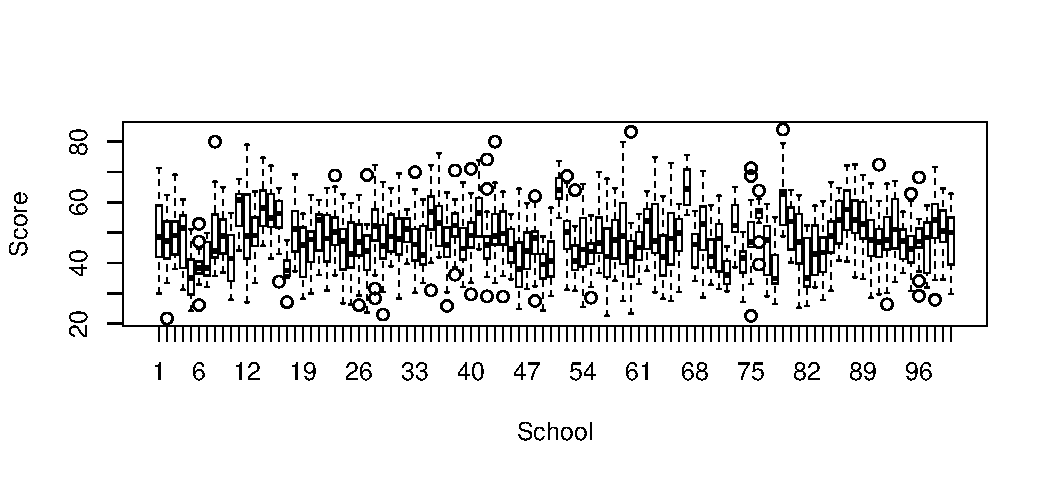
\includegraphics[width=\maxwidth]{figure/unnamed-chunk-1-1} 
\begin{kframe}\begin{alltt}
\hlstd{school.avgs} \hlkwb{<-} \hlkwd{aggregate}\hlstd{(data,} \hlkwd{list}\hlstd{(}\hlkwc{school}\hlstd{=school), mean)[,}\hlnum{3}\hlstd{]}
\hlstd{school.ssize} \hlkwb{<-} \hlkwd{aggregate}\hlstd{(data,} \hlkwd{list}\hlstd{(}\hlkwc{school}\hlstd{=school), length)[,}\hlnum{3}\hlstd{]}
\hlkwd{plot}\hlstd{(}\hlkwd{cbind}\hlstd{(school.avgs, school.ssize))}
\hlstd{fit} \hlkwb{<-} \hlkwd{lowess}\hlstd{(}\hlkwd{cbind}\hlstd{(school.avgs, school.ssize))}
\hlkwd{lines}\hlstd{(fit)}
\end{alltt}
\end{kframe}
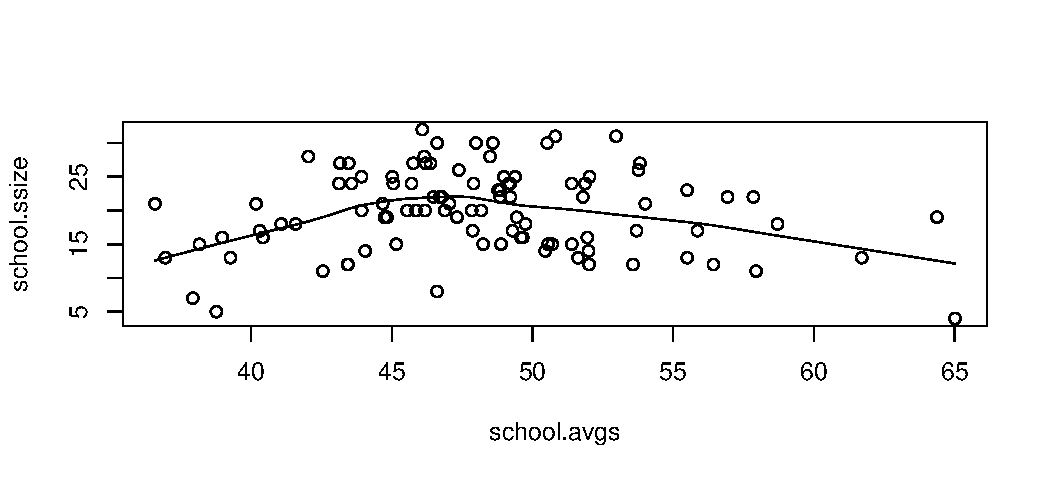
\includegraphics[width=\maxwidth]{figure/unnamed-chunk-1-2} 

\end{knitrout}

\subsection{Normal Hierarchical Model with Gibbs Sampling}

\subsubsection{Model}
For school $i=1,\cdots,p$; student $j=1,\cdots,n_i$; and $\sum n_i = n$; 
let $a=b=c=d=1$, and note that for this data, $p=100$ and $n=1993$:
\begin{align*}
  y_{ij} &\sim\ N(\theta_i,\sigma^2)\\
  \theta_i &\sim\ N(\mu,\tau^2)\\
  \mu &\sim\ N(m, v)\\
  \sigma^2 &\sim\ InvGa(a,b)\\
  \tau^2 &\sim\ InvGa(c,d)\\
\end{align*}

\subsubsection{Joint and Posterior Distributions}

See attached sheets.

\subsubsection{Gibbs Sampler}

The Gibbs Sampler produces the following results. Immediately below are the posterior estimates for $\theta$.

\begin{knitrout}
\definecolor{shadecolor}{rgb}{0.969, 0.969, 0.969}\color{fgcolor}\begin{kframe}
\begin{verbatim}
##   [1] 50.51003 46.76601 48.68838 47.46504 38.42135 40.81311 41.92385
##   [8] 48.75465 49.04415 42.40514 55.54075 50.25178 49.24118 57.04885
##  [15] 54.38310 54.39402 41.56460 49.98703 44.52868 46.26326 50.21306
##  [22] 47.97774 51.22848 46.00253 45.33894 46.74912 44.53177 51.34644
##  [29] 46.61217 49.30503 49.06949 49.95425 47.46797 46.04563 54.34171
##  [36] 52.19013 46.37511 51.15531 46.49257 48.86489 55.62025 46.38389
##  [43] 50.77899 49.03702 45.82999 41.40744 44.73532 47.10874 40.19376
##  [50] 42.70538 61.67738 49.22951 43.98558 46.66859 43.88010 49.12179
##  [57] 44.37257 48.45245 49.51989 42.84086 45.46777 50.88362 49.35530
##  [64] 43.80215 48.00024 48.28518 56.62764 45.40195 51.38905 43.95266
##  [71] 46.98120 39.64060 53.07232 41.71179 48.77520 53.80514 45.19835
##  [78] 41.35697 58.58670 51.00293 47.14796 42.88651 44.88587 44.21317
##  [85] 48.70792 52.64602 56.46694 53.17146 53.07175 48.53131 47.88498
##  [92] 48.07271 51.49883 47.06121 45.36017 47.18530 46.13284 52.52240
##  [99] 51.05314 48.09516
\end{verbatim}
\end{kframe}
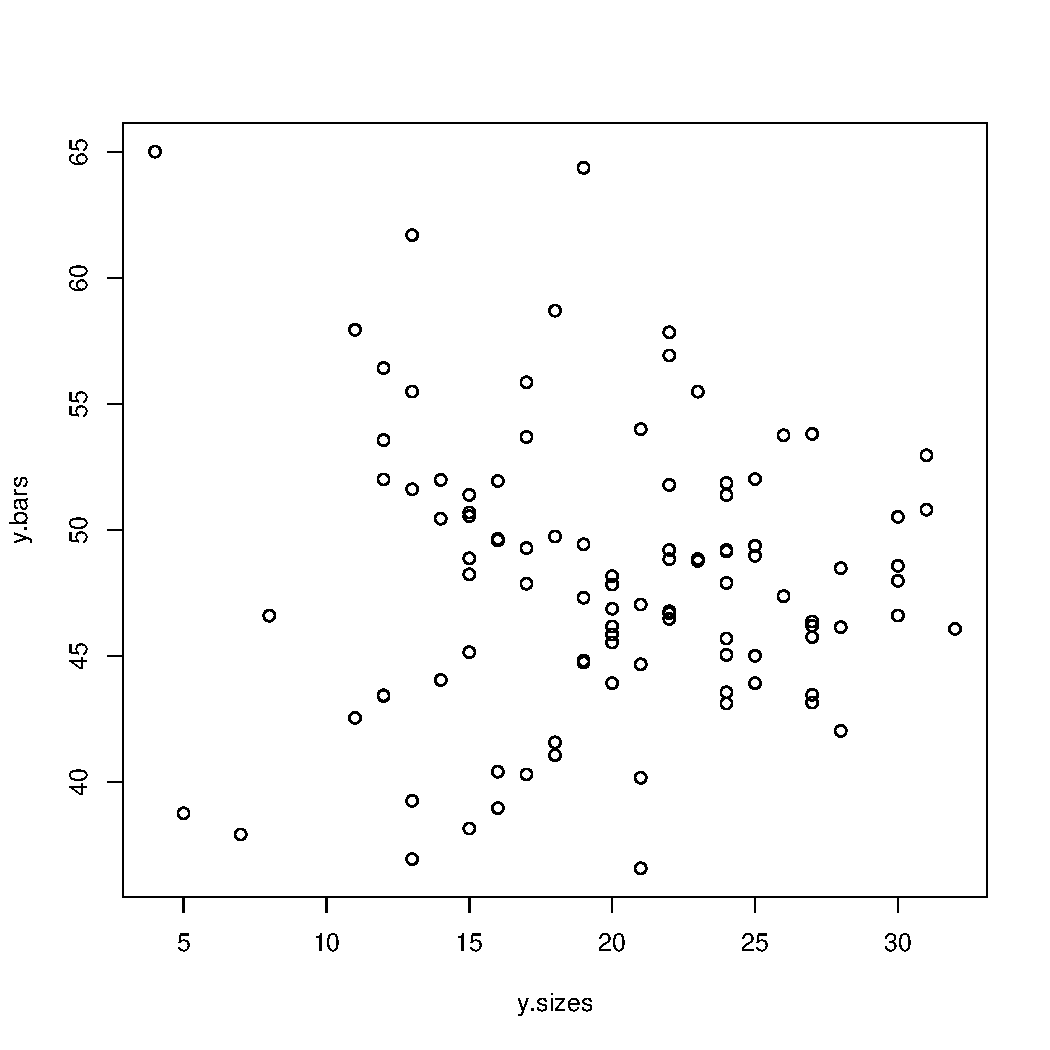
\includegraphics[width=\maxwidth]{figure/unnamed-chunk-2-1} 

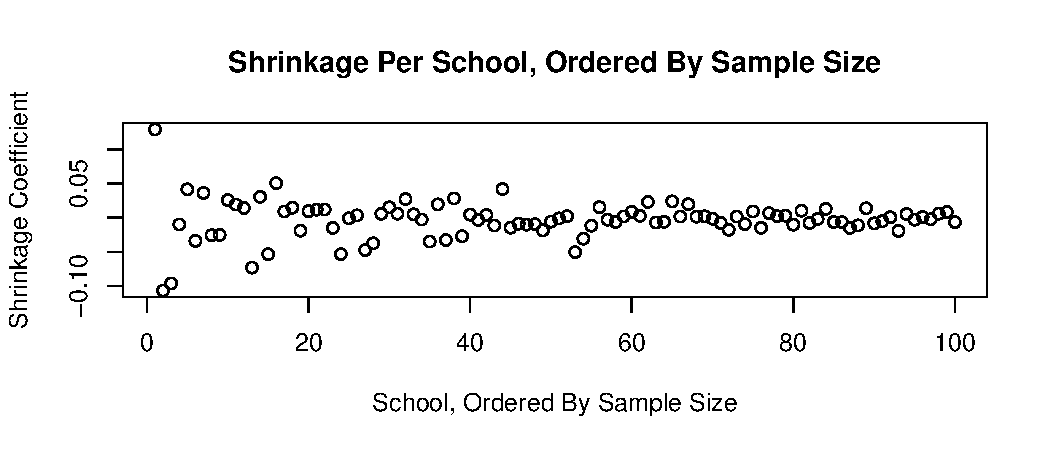
\includegraphics[width=\maxwidth]{figure/unnamed-chunk-2-2} 

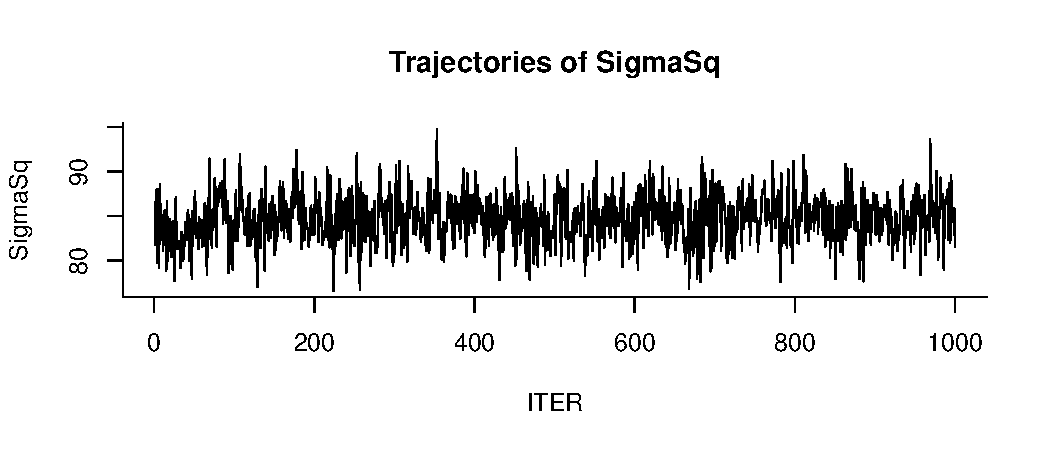
\includegraphics[width=\maxwidth]{figure/unnamed-chunk-2-3} 

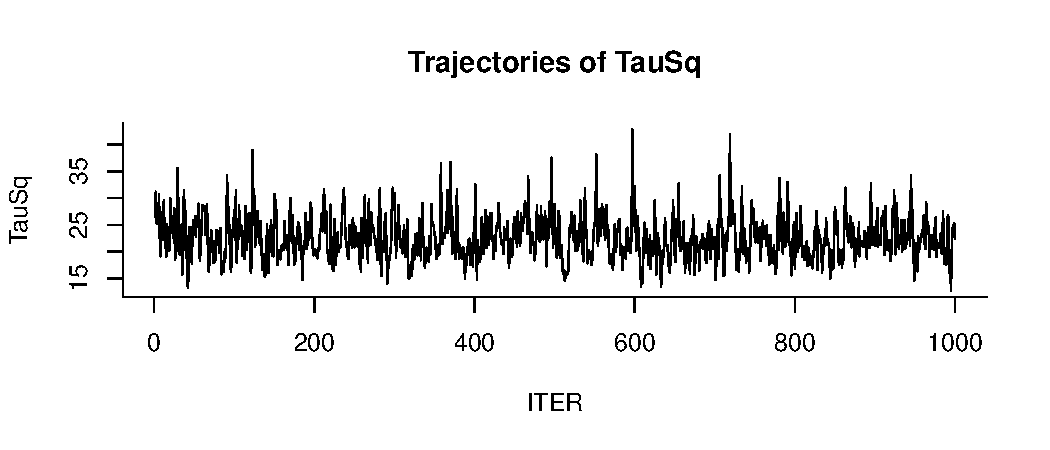
\includegraphics[width=\maxwidth]{figure/unnamed-chunk-2-4} 

\end{knitrout}

\subsection{Shrinkage}

In general, the smaller the sample size, the more extreme the sample mean, and the larger the shrinkage coefficient. 

\end{document}

